\begin{frame}
  \frametitle{Baby (the SSEM) and its Program}
  \begin{columns}
    \column[T]{0.6\linewidth}
    \begin{figure}
      \centering
      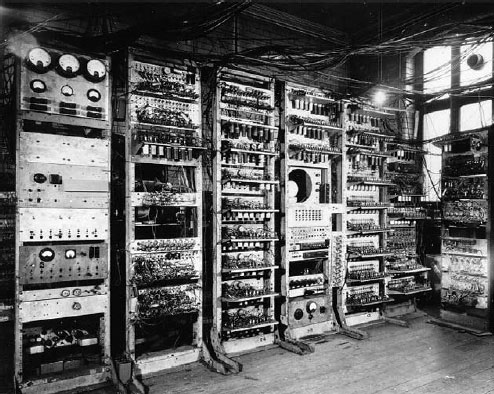
\includegraphics[width=0.73\linewidth]{Graphics/SSEM.jpg}
      \caption{The Small-Scale Experimental Machine (SSEM) computing system nicknamed \emph{Baby} started with a glowing bit on a screen controlled by an electron beam and grew to a vacuum tube-filled system to control \num{1024} bits for a simple calculation}
      \label{fig:Baby}
    \end{figure}

  \column[T]{0.4\linewidth}
    \begin{figure}
      \centering
      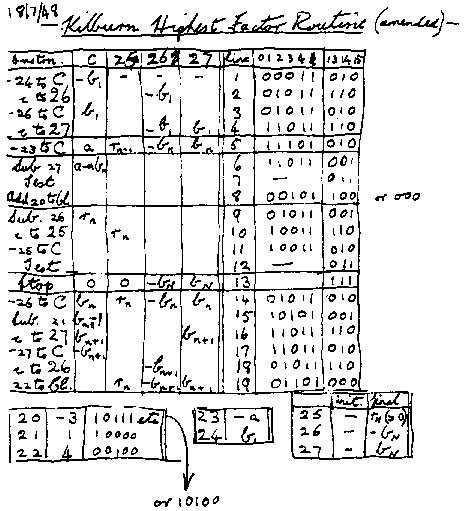
\includegraphics[width=0.9\linewidth]{Graphics/first_prog.jpg}
      \caption{\emph{Baby}'s first program --- 7 instructions to find highest proper divisor of a number}
      \label{fig:Baby-1st-program}
    \end{figure}  
  \end{columns}
\end{frame}
